% =============================================================================
%  Data engineering report — Project 1: WHO SDG 3 indicators (EN)
%  Build: latexmk -xelatex report-en.tex   (see README.md in this folder)
% =============================================================================
\documentclass[11pt, a4paper, oneside, headings=normal, numbers=noenddot, DIV=12]{scrartcl}
\usepackage[english]{babel}
\usepackage{report-style}
\graphicspath{{../livraison/figures/en/}}
\sisetup{group-separator={,}, group-minimum-digits=4}

% --- Acceptance results (filled in after the fresh-environment run) -----------
\newcommand{\RecInstall}{57\,s}
\newcommand{\RecPipeline}{2\,min 43\,s (real extraction included)}
\newcommand{\RecRows}{129,368}

% --- Metadata ----------------------------------------------------------------
\newcommand{\ReportAuthor}{LUMU BAMANA MANASSE}
\newcommand{\ReportAuthorRole}{Data engineer}
\newcommand{\ReportShortTitle}{WHO SDG 3 indicators · Data engineering report}
\newcommand{\ReportFooter}{October 2026 · v1.0.0}
\newcommand{\ReportKicker}{Data engineering report · Project 1}
\newcommand{\ReportTitle}{Global health:\\SDG 3 in Africa}
\newcommand{\ReportSubtitle}{A reliable PostgreSQL warehouse of WHO indicators:\\ingestion, quality, upsert and 2030 target analysis}
\newcommand{\ReportMeta}{%
  \begin{tabularx}{\linewidth}{@{}>{\bfseries}l@{\hspace{1em}}Y@{}}
  Date & October 2026 \\
  Version & 1.0.0 (delivered and accepted) \\
  Client & Initiative Baobab Santé (fictional NGO) · Engagement IBS-2026-001 \\
  GitHub repository & \url{https://github.com/MediJr/who-sdg3-health-etl} \\
  Language & English · \textit{version française disponible dans le dépôt}
  \end{tabularx}}
\newcommand{\ReportScenario}{Fictional scenario, real data: the client NGO and its staff are invented to simulate a complete professional
  engagement. The data comes from the WHO Global Health Observatory, extracted on 22 October 2026. This project is not commissioned,
  endorsed by or affiliated with the World Health Organization.}
\hypersetup{pdftitle={Global health: SDG 3 in Africa, data engineering report}, pdfauthor={Lumu Bamana Manasse},
  pdfsubject={WHO ETL pipeline to PostgreSQL, portfolio project}, pdflang={en-US}}

\begin{document}
\sloppy   % césure anglaise moins souple : on autorise un espacement un peu plus large
\MakeTitlePage

% =============================================================================
\section*{Document control}
\addcontentsline{toc}{section}{Document control}

\begin{tabularx}{\linewidth}{@{}>{\bfseries\sffamily}L{4.2cm}Y@{}}
\toprule
Project & Portfolio project 1: PostgreSQL warehouse of WHO health indicators \\
Engagement & IBS-2026-001: ``Monitor SDG 3 in Africa with WHO data'' \\
Client & Initiative Baobab Santé, maternal and child health NGO (fictional), attn. Dr Mariam Koné \\
Author & Lumu Bamana Manasse, data engineer \\
Delivery period & October 2026 \\
Data & WHO GHO API, batch of 22 October 2026 \\
Status & \pill{good}{DELIVERED} \pill{good}{ACCEPTED} \\
Source code & \url{https://github.com/MediJr/who-sdg3-health-etl} \\
\bottomrule
\end{tabularx}

\subsection*{Version history}
\begin{tabularx}{\linewidth}{@{}l l Y@{}}
\toprule
\textbf{Version} & \textbf{Date} & \textbf{Description} \\
\midrule
0.1 & 2026-10-22 & Scoping: brief, meeting minutes, statement of work \\
0.9 & 2026-10-22 & Pipeline, tests, analyses, fixes (quality, performance) \\
1.0.0 & 2026-10-22 & Fresh-environment acceptance, final report (French and English) \\
\bottomrule
\end{tabularx}

\subsection*{Reading guide}
\begin{tabularx}{\linewidth}{@{}>{\bfseries}L{4.2cm}Y@{}}
Board of directors & \hyperref[sec:summary]{1. Executive summary} and \hyperref[sec:results]{11. Results and recommendations} \\
Monitoring \& evaluation lead & 2. Scoping, 6. Data model, 7. Data quality, 12. Limitations \\
Engineer taking over & 4. Architecture, 5. Pipeline, 9. Operations, 10. Testing, appendices \\
\end{tabularx}

\begingroup
\addtokomafont{sectionentry}{\color{primary}}
\setcounter{tocdepth}{2}
\tableofcontents
\endgroup
\clearpage

% =============================================================================
\section{Executive summary}\label{sec:summary}

\textbf{The need.} The NGO Initiative Baobab Santé tracks African countries' progress towards the SDG 3 targets every year.
Its process was manual (downloads, copy-pasting into Excel), not reproducible, and had already led to an error presented to the board:
a table mixed several data categories without anyone noticing.

\textbf{The solution.} A Python pipeline automatically feeds a containerised \textbf{PostgreSQL} warehouse with 9 WHO indicators.
The grain is explicit, quality checks quarantine invalid rows, and an \textbf{upsert} load applies WHO revisions without ever creating
duplicates. The client's team queries the database in SQL.

\kpirow{129,368}{WHO\\observations}{9}{SDG 3\\indicators}{386}{locations (countries,\\regions, world)}{22 / 22}{automated\\tests}
\kpirow{0 / 0}{inserts / updates\\on re-run}{10 s}{full\\reload}{×15}{speed-up\\after diagnosis}{0}{personal\\data}

\begin{keybox}[Key findings for the WHO African Region (47 countries)]
\begin{itemize}[leftmargin=1.2em]
  \item \textbf{Q1 · 2030 targets:} only \textbf{5 of 47 countries} have met the under-five mortality target (25 per 1,000), and 4 the maternal
        mortality target (70 per 100,000). The region remains far behind the global average.
  \item \textbf{Q2 · Pace:} \textbf{no} off-target country is on track to meet the under-five mortality goal by 2030. The median country
        reduces it by 3.0\% a year, but would need 12.4\%: \textbf{four times faster}.
  \item \textbf{Q3 · Inequality:} a child from the poorest 20\% of households is \textbf{1.7 times more likely} to die before age 5
        (up to 2.5 times in Nigeria). The absolute gap is shrinking, but the relative gap has widened since 2000.
  \item \textbf{Q4 · Inputs:} \textbf{skilled birth attendance} is the input most strongly associated with low mortality (correlation of $-0.75$).
\end{itemize}
\end{keybox}

\textbf{What this project demonstrates on the engineering side:} a containerised PostgreSQL database, secrets kept out of the code, a layered
model (staging, core, ops), a complete business key with \texttt{NULLS NOT DISTINCT}, bulk loading with \texttt{COPY} followed by an idempotent and
measurable upsert, quality checks with quarantine, a run log, unit and integration tests, and two production diagnoses: a Docker outage and a
130-second connection brought down to zero.

% =============================================================================
\section{Context and scoping}

\subsection{The client's real problems}
Analysis of the brief showed that the client's problem was first a \textbf{data engineering} problem, and only then an analytics one:

\begin{table}[H]
\centering\small
\begin{tabularx}{\linewidth}{@{}L{4.4cm} Y@{}}
\toprule
\textbf{Symptom described by the client} & \textbf{Technical cause} \\
\midrule
``We download the tables by hand'' & No reproducible or traceable process \\
``The numbers never match from one year to the next'' & WHO revises its estimates, and nobody keeps track of revisions \\
``A table mixed several categories'' & \textbf{Grain error}: the same country-year value exists by sex, age and wealth quintile \\
\bottomrule
\end{tabularx}
\caption{From symptom to cause}
\end{table}

\subsection{Business questions}
\begin{table}[H]
\centering
\begin{tabularx}{\linewidth}{@{}l Y L{4.2cm}@{}}
\toprule
\textbf{\#} & \textbf{Question} & \textbf{Decision supported} \\
\midrule
Q1 & Where do African Region countries stand against the 2030 SDG 3 targets? & Diagnosis presented to the board \\
Q2 & At their current pace, which countries will meet the targets by 2030? & Prioritising countries to fund \\
Q3 & How large is the child mortality gap between the poorest and richest households? & Programme targeting \\
Q4 & Are health system inputs associated with better outcomes? & Choice of levers \\
\bottomrule
\end{tabularx}
\caption{Questions agreed during scoping}
\end{table}

\subsection{Technical requirements}
\begin{table}[H]
\centering\small
\begin{tabularx}{\linewidth}{@{}L{5.6cm} Y@{}}
\toprule
\textbf{Requirement} & \textbf{Technical answer} \\
\midrule
SQL access for several users & PostgreSQL 17 in Docker \\
Re-runnable at any time, no duplicates & Upsert on a complete business key \\
Latest published value, and revision date & \texttt{last\_changed\_at}, \texttt{last\_run\_id} \\
Explicit grain & \texttt{UNIQUE NULLS NOT DISTINCT} key on 7 columns \\
Checks before loading & 9 rules and a quarantine table \\
Passwords out of the code & \texttt{.env} file excluded from Git \\
Automated tests & \texttt{pytest}: 17 unit tests and 5 integration tests \\
\bottomrule
\end{tabularx}
\caption{Statement of work requirements and how they were met}
\end{table}

\subsection{Scope}
The database holds the 9 indicators for \textbf{all countries and regions} published by WHO, so it is reusable beyond this engagement.
The analyses focus on the \textbf{WHO African Region} (47 countries with data), with the global value as a benchmark.

% =============================================================================
\section{Data sources}

\begin{table}[H]
\centering\small
\begin{tabularx}{\linewidth}{@{}L{3.4cm} Y L{3.6cm}@{}}
\toprule
\textbf{GHO resource} & \textbf{Content} & \textbf{Volume (22 Oct batch)} \\
\midrule
\texttt{/api/\{indicator\}} & Observations: value, uncertainty bounds, update date & 129,368 rows, 9 indicators \\
\texttt{/api/Indicator} & Official indicator names & 9 rows \\
\texttt{/api/DIMENSION/}\allowbreak\texttt{\{type\}/}\allowbreak\texttt{DimensionValues} & Location and breakdown labels & 386 locations, 174 breakdowns \\
\bottomrule
\end{tabularx}
\caption{WHO API resources used (OData protocol, no API key)}
\end{table}

\begin{table}[H]
\centering\small
\begin{tabularx}{\linewidth}{@{}l Y r l@{}}
\toprule
\textbf{Code} & \textbf{Indicator} & \textbf{Rows} & \textbf{2030 target} \\
\midrule
\texttt{MDG\_0000000007} & Under-five mortality (per 1,000) & 64,510 & $\leq 25$ \\
\texttt{WHOSIS\_000001} & Life expectancy at birth & 14,112 & – \\
\texttt{WHOSIS\_000002} & Healthy life expectancy & 14,112 & – \\
\texttt{WHOSIS\_000003} & Neonatal mortality (per 1,000) & 12,128 & $\leq 12$ \\
\texttt{MDG\_0000000026} & Maternal mortality (per 100,000) & 7,878 & $< 70$ \\
\texttt{WHS4\_100} & DTP3 immunisation coverage (\%) & 5,337 & 90\% \\
\texttt{GHED\_CHE\_pc\_US\_SHA2011} & Health expenditure per capita (USD) & 4,849 & – \\
\texttt{HWF\_0001} & Doctors per 10,000 & 3,693 & – \\
\texttt{MDG\_0000000025} & Skilled birth attendance (\%) & 2,749 & – \\
\bottomrule
\end{tabularx}
\caption{Indicators collected}
\end{table}

\begin{keybox}[Key exploration finding: the hidden dimension]
For Senegal in 2020, under-five mortality appears \textbf{8 times with 8 different values}, from 27.9 to 61.2 per 1,000.
These are not duplicates: the \texttt{Dim3} column carries the \textbf{wealth quintile} (61 per 1,000 for the poorest 20\% of households,
28 for the richest 20\%). This is exactly the mistake the client made the year before. The finding set the \textbf{grain} of the fact table
and gave rise to question Q3.
\end{keybox}

% =============================================================================
\section{Solution architecture}

\begin{figure}[H]
\centering
\resizebox{\linewidth}{!}{%
\begin{tikzpicture}[
  font=\sffamily\small, node distance=0.6cm and 0.8cm,
  src/.style={draw=rule, fill=panel, rounded corners=2pt, minimum width=2.4cm, minimum height=1.2cm, align=center},
  stage/.style={draw=primary, fill=primary, text=white, rounded corners=3pt, minimum width=2.4cm, minimum height=1.2cm, align=center, font=\sffamily\small\bfseries},
  store/.style={cylinder, shape border rotate=90, aspect=0.18, draw=accent, fill=accent!8, minimum width=2.2cm, minimum height=1.4cm, align=center},
  bad/.style={cylinder, shape border rotate=90, aspect=0.18, draw=warn, fill=warn!8, minimum width=2.2cm, minimum height=1.2cm, align=center},
  deliv/.style={draw=accent, rounded corners=2pt, minimum width=2.4cm, minimum height=0.7cm, align=center},
  arr/.style={-{Stealth[length=2.6mm]}, thick, color=ink2}]
  \node[src] (api) {WHO API\\\scriptsize GHO (OData)};
  \node[stage, right=of api] (e) {EXTRACT\\\scriptsize\mdseries retries · gzip · SHA-256};
  \node[store, below=0.9cm of e] (raw) {\scriptsize data/raw/\\\scriptsize YYYY-MM-DD};
  \node[stage, right=of e] (t) {TRANSFORM\\\scriptsize\mdseries grain · 9 checks};
  \node[bad, above=0.7cm of t] (q) {\scriptsize ops.\\\scriptsize quarantine};
  \node[stage, right=1.5cm of t] (l) {LOAD\\\scriptsize\mdseries COPY → UPSERT};
  \node[store, right=of l, minimum height=1.9cm] (db) {\scriptsize PostgreSQL 17\\\scriptsize staging · core · ops\\\scriptsize (Docker)};
  \node[deliv, right=0.9cm of db, yshift=0.9cm] (o1) {SQL views};
  \node[deliv, below=0.25cm of o1] (o2) {Client team};
  \node[deliv, below=0.25cm of o2] (o3) {Report};
  \draw[arr] (api) -- (e);
  \draw[arr] (e) -- (raw);
  \draw[arr] (raw.east) -| (t.south);
  \draw[arr] (t) -- node[right, font=\scriptsize\sffamily, text=warn]{invalid} (q);
  \draw[arr] (t) -- node[above, font=\scriptsize\sffamily, text=ink2]{valid} (l);
  \draw[arr] (l) -- (db);
  \foreach \o in {o1,o2,o3} \draw[arr] (db.east) -- (\o.west);
  \begin{scope}[on background layer]
    \node[draw=rule, dashed, rounded corners=6pt, fit=(e)(t)(l)(raw)(q), inner sep=9pt, label={[font=\scriptsize\sffamily, text=ink2]above:python -m src.pipeline}] {};
  \end{scope}
\end{tikzpicture}}
\caption{Architecture: one command collects, checks and loads the data into PostgreSQL}
\end{figure}

\subsection{Technology choices}
\begin{table}[H]
\centering\small
\begin{tabularx}{\linewidth}{@{}L{2.6cm} L{3.2cm} Y@{}}
\toprule
\textbf{Need} & \textbf{Choice} & \textbf{Rationale} \\
\midrule
Database & PostgreSQL 17 & Multi-user, strong constraints, native upsert, \texttt{NULLS NOT DISTINCT} (ADR 001) \\
Running the database & Docker Compose & Same database on every machine, one command, no manual install \\
Driver & psycopg 3 & Modern driver, \texttt{COPY} for bulk loading \\
Secrets & python-dotenv + \texttt{.env} & No password in the code or in Git \\
HTTP retries & \texttt{urllib3.Retry} & Exponential back-off, honours the \texttt{Retry-After} header \\
Tests & pytest & Unit tests without a database, integration tests on a dedicated database \\
\bottomrule
\end{tabularx}
\caption{Technology stack (on top of Python, pandas and matplotlib, already used in project 0)}
\end{table}

\subsection{What changed since project 0}
\begin{table}[H]
\centering\small
\begin{tabularx}{\linewidth}{@{}L{3.2cm} Y Y@{}}
\toprule
& \textbf{Project 0} & \textbf{Project 1} \\
\midrule
Database & DuckDB (file) & PostgreSQL (server, container) \\
Loading & Full refresh & Staging + upsert, data kept across runs \\
Idempotency & Guaranteed by replacement & \textbf{Measured}: inserted / updated / unchanged counters \\
Quality & Checks after the fact & Checks \textbf{before} loading, plus quarantine \\
Secrets & None & \texttt{.env} file \\
Tests & Manual acceptance & 22 automated tests \\
Traceability & Manifest & Manifest with SHA-256, and a run log in the database \\
\bottomrule
\end{tabularx}
\caption{Portfolio progression}
\end{table}

% =============================================================================
\section{Pipeline design}

\subsection{Extraction}
\begin{itemize}[leftmargin=1.2em]
  \item \textbf{Retries delegated to \texttt{urllib3.Retry}}: up to 4 attempts, waiting 2, 4, 8 and 16\,s, on transient errors only
        (429, 500, 502, 503, 504) and never on a 404.
  \item \textbf{OData pagination followed} (\texttt{@odata.nextLink}), and \textbf{explicit failure} if the response lacks the \texttt{value}
        key: better to crash than to load anything.
  \item \textbf{Compressed raw layer} (gzip, 6.4\,MB for 129,368 rows) with \textbf{atomic writes}.
  \item \textbf{Manifest} with the SHA-256 fingerprint of each file, proving the batch's integrity.
\end{itemize}

\subsection{Transformation and quality checks}
Breakdowns are mapped by their \textbf{declared type} (\texttt{Dim1Type}, \texttt{Dim2Type}…), never by position: WHO may put sex in the
first or second dimension depending on the indicator. Nine rules are then applied:

\begin{table}[H]
\centering\small
\begin{tabularx}{\linewidth}{@{}l Y@{}}
\toprule
\textbf{\#} & \textbf{Rule (quarantine reason)} \\
\midrule
1 & Indicator not in the reference list \\
2 & Missing or non-numeric value \\
3 & Value outside plausibility bounds (logical limits, see section 7) \\
4 & Inconsistent uncertainty interval (lower bound > value, or value > upper bound) \\
5 & Invalid year \\
6 & Unknown location \\
7 & Unknown breakdown value \\
8 & Unknown breakdown type \\
9 & Duplicate business key within the batch \\
\bottomrule
\end{tabularx}
\caption{Quality rules applied before loading}
\end{table}

\subsection{Loading: staging and upsert}
The batch is bulk-copied into \texttt{staging.}\allowbreak\texttt{observation} (\texttt{COPY}, 0.9\,s), then merged into \texttt{core.}\allowbreak\texttt{fact\_observation} by
a single query:

\begin{lstlisting}[language=DuckSQL]
INSERT INTO core.fact_observation AS f (...)
SELECT ... FROM staging.observation
ON CONFLICT ON CONSTRAINT uq_observation_business_key DO UPDATE SET
    value = EXCLUDED.value, value_low = EXCLUDED.value_low, value_high = EXCLUDED.value_high,
    last_changed_at = now(), last_run_id = EXCLUDED.last_run_id
WHERE (f.value, f.value_low, f.value_high)
      IS DISTINCT FROM (EXCLUDED.value, EXCLUDED.value_low, EXCLUDED.value_high)
RETURNING (xmax = 0) AS inserted      -- true: inserted, false: updated
\end{lstlisting}

\begin{itemize}[leftmargin=1.2em]
  \item \texttt{ON CONFLICT}: if the business key already exists, update instead of insert.
  \item \texttt{WHERE … IS DISTINCT FROM}: only values actually revised by WHO are touched.
  \item \texttt{IS DISTINCT FROM} rather than \texttt{<>}: it compares \texttt{NULL}s correctly, which \texttt{<>} does not.
  \item Merge, quarantine and run log are committed in \textbf{a single transaction}. The run log entry is opened separately, so that a failure
        remains on record.
\end{itemize}

% =============================================================================
\section{Data model}

\begin{figure}[H]
\centering
\resizebox{0.97\linewidth}{!}{%
\begin{tikzpicture}[font=\sffamily\scriptsize,
  ent/.style={draw=primary, fill=white, rounded corners=2pt, align=left, inner sep=5pt},
  ops/.style={draw=ink2, dashed, fill=white, rounded corners=2pt, align=left, inner sep=5pt},
  rel/.style={-{Stealth[length=2mm]}, thick, color=accent}]
  \node[ent, minimum width=5.2cm] (f) {\textbf{\normalsize core.fact\_observation}\\[2pt]
     \textbf{business key:} indicator\_code, location\_type, location\_code,\\year, sex, age\_group, wealth\_quintile\\[2pt]
     value, value\_low, value\_high, who\_updated\_at\\first\_loaded\_at, last\_changed\_at, last\_run\_id};
  \node[ent, above left=0.6cm and 0.4cm of f] (i) {\textbf{\normalsize dim\_indicator}\\\textbf{indicator\_code}\\name\_fr, unit, role\\target\_2030, target\_direction};
  \node[ent, above right=0.6cm and 0.4cm of f] (l) {\textbf{\normalsize dim\_location}\\\textbf{location\_type, location\_code}\\name, who\_region};
  \node[ent, below left=0.6cm and 0.4cm of f] (b) {\textbf{\normalsize dim\_breakdown}\\\textbf{breakdown\_code}\\breakdown\_type, label};
  \node[ops, below right=0.6cm and 0.4cm of f] (r) {\textbf{\normalsize ops.pipeline\_run}\\\textbf{run\_id}\\rows\_inserted / updated\\unchanged / quarantined};
  \node[ops, right=0.6cm of r] (q) {\textbf{\normalsize ops.quarantine}\\run\_id, reason\\raw\_record (JSON)};
  \draw[rel] (f) -- (i); \draw[rel] (f) -- (l); \draw[rel] (f) -- node[left, font=\scriptsize]{×3} (b); \draw[rel] (f) -- (r); \draw[rel] (q) -- (r);
\end{tikzpicture}}
\caption{Data model (core and ops schemas; arrows represent foreign keys)}
\end{figure}

\begin{keybox}[Why NULLS NOT DISTINCT?]
By default in SQL, \texttt{NULL = NULL} is not true: two ``no breakdown'' rows are not considered duplicates, so a regular unique constraint
would let through endless copies. \texttt{UNIQUE NULLS NOT DISTINCT} (PostgreSQL 15+) treats \texttt{NULL}s as equal and closes that gap.
\end{keybox}

\textbf{Analysis views.} \texttt{core.v\_national} encapsulates the grain rule (both sexes, no wealth breakdown) and \texttt{core.v\_latest}
returns the latest available year. The client's team no longer needs to know these rules to get a correct value.

% =============================================================================
\section{Data quality}

\subsection{Coverage}
All 9 indicators are available for the \textbf{47 countries} of the African Region with data (out of 50 country and territory codes).
The data is recent: 2023 to 2025 depending on the indicator. The one exception is skilled birth attendance, for which only 32 countries have
data after 2020 (median: 2021).

\subsection{Threshold calibration: a lesson from real-world data}
On the first run, ``intuitive'' plausibility thresholds sent \textbf{25 rows to quarantine}. Reviewing them showed they were not errors,
but the statistical traces of major humanitarian crises:

\begin{table}[H]
\centering\small
\begin{tabularx}{\linewidth}{@{}L{4.6cm} r Y@{}}
\toprule
\textbf{Initial threshold} & \textbf{Rows} & \textbf{What these values were} \\
\midrule
Under-five mortality ≤ 500 per 1,000 & 18 & Cambodia 1975–1978 (Khmer Rouge regime), South Sudan 1988, Iraq 1942–1944 \\
Maternal mortality ≤ 5,000 & 7 & Rwanda 1994 (genocide), South Sudan 1987–1998 (civil war) \\
\bottomrule
\end{tabularx}
\caption{Extreme but real values, wrongly quarantined}
\end{table}

The thresholds were replaced by \textbf{logical limits}: a rate per 1,000 births cannot exceed 1,000, a percentage cannot exceed 100 (ADR 003).
Result: \textbf{129,368 valid rows, 0 quarantined}, while the checks still block genuine errors, as the tests prove.

\begin{keybox}[Lesson]
A quality rule must be calibrated with domain knowledge. The quarantine did its job: isolating suspicious values for human review, instead of
silently deleting them or loading them unexamined.
\end{keybox}

% =============================================================================
\section{Security and governance}

\begin{tabularx}{\linewidth}{@{}L{3.6cm} Y@{}}
\toprule
\textbf{Topic} & \textbf{Measure} \\
\midrule
Secrets & PostgreSQL credentials in \texttt{.env} (excluded from Git). A secret-free template, \texttt{.env.example}, is versioned. Random password generated locally. \\
Network exposure & Database reachable from the local machine only (\texttt{127.0.0.1:5433}) \\
Personal data & None: WHO data is aggregated at country level \\
Data licence & WHO data used under its data policy, for non-commercial purposes, with source attribution \\
Traceability & SHA-256 manifest, \texttt{ops.pipeline\_run} log, \texttt{last\_run\_id} on every observation, ADRs, work log \\
\bottomrule
\end{tabularx}

% =============================================================================
\section{Operations}

\subsection{Commands}
\begin{lstlisting}[language=bash]
copy .env.example .env                         # then choose a password
docker compose up -d                           # starts PostgreSQL (port 5433)
pip install -r requirements.txt
python -m src.pipeline                         # extraction + loading + report
python -m src.pipeline --run-date 2026-10-22   # replay a raw batch, no API calls
pytest                                         # 22 tests (5 on a dedicated database)
\end{lstlisting}

\subsection{Production diagnoses}
Two real incidents were diagnosed and resolved during the engagement:

\begin{table}[H]
\centering\small
\begin{tabularx}{\linewidth}{@{}L{3cm} Y Y@{}}
\toprule
\textbf{Incident} & \textbf{Diagnosis} & \textbf{Resolution} \\
\midrule
Docker Desktop crashes on start-up & Backend log: two Unix sockets (\texttt{sailor-ingest.sock}, \texttt{engine.sock}) locked since a hard shutdown a month earlier & Folders renamed (nothing deleted). Docker recreates clean folders. \\
\midrule
156\,s to load 129,368 rows & Step-by-step timing: \texttt{COPY} 0.9\,s, upsert 2.8\,s, but \textbf{connection 130\,s}. \texttt{localhost} resolves to IPv6 (\texttt{::1}) first, where Docker does not listen. & Host \texttt{127.0.0.1} and \texttt{connect\_timeout=10}: pipeline in \textbf{10\,s} (×15) \\
\bottomrule
\end{tabularx}
\caption{Incidents resolved}
\end{table}

\begin{keybox}[Lesson]
Measure instead of guessing: the bottleneck was neither in the Python code nor in PostgreSQL, but in host name resolution.
\end{keybox}

% =============================================================================
\section{Testing and acceptance}

\subsection{Automated tests}
\begin{table}[H]
\centering\small
\begin{tabularx}{\linewidth}{@{}L{4.3cm} r Y@{}}
\toprule
\textbf{File} & \textbf{Tests} & \textbf{What is checked} \\
\midrule
\texttt{test\_extract.py} & 4 & OData pagination, failure on unexpected structure, atomic write, retries limited to transient errors \\
\texttt{test\_transform.py} & 13 & Grain (distinct quintiles), breakdowns mapped by type, each quarantine rule, no row lost \\
\texttt{test\_load\_integration.py} & 5 & On a real dedicated database: first load, idempotent re-run, revision detected, quarantine stored, unique constraint \\
\bottomrule
\end{tabularx}
\caption{22 tests, on a real API extract (Senegal, 2020)}
\end{table}

The tests found a \textbf{real bug}: in a mixed pandas column, \texttt{None} becomes \texttt{NaN}, and \texttt{NaN} is ``truthy'' in Python.
A single row with an unknown breakdown then sent \textbf{every} row to quarantine.

\subsection{Fresh-environment acceptance}
Copy of the publishable files only, a new Python environment, \texttt{.env} recreated from the template, a \textbf{blank PostgreSQL database},
and a real extraction from the API.

\begin{table}[H]
\centering\small
\begin{tabularx}{\linewidth}{@{}l L{4.6cm} Y c@{}}
\toprule
\textbf{\#} & \textbf{Criterion} & \textbf{Result} & \\
\midrule
C1 & End-to-end run, database included & Install in \RecInstall, pipeline in \RecPipeline & \ok \\
C2 & Re-run with no duplicate or change & 0 inserted, 0 updated, \RecRows{} unchanged & \ok \\
C3 & Business key covering every dimension & Database constraint, 0 duplicates, integration test & \ok \\
C4 & Invalid rows quarantined, never lost & Invariant extracted = loaded + quarantined & \ok \\
C5 & No secret in the repository & \texttt{.env} excluded, no password in versioned files & \ok \\
C6 & Test suite fully green & 22 / 22 & \ok \\
C7 & One query and one answer per question & Section~\ref{sec:results} & \ok \\
\bottomrule
\end{tabularx}
\caption{Acceptance results (details: \texttt{docs/livraison/2026-10-22-pv-recette.md}, in French)}
\end{table}

% =============================================================================
\section{Results and recommendations}\label{sec:results}

\subsection{Q1 · Where do countries stand against the 2030 targets?}

\begin{table}[H]
\centering\small
\begin{tabularx}{\linewidth}{@{}Y r r r r@{}}
\toprule
\textbf{Indicator} & \textbf{Target} & \textbf{Countries on target} & \textbf{Africa median} & \textbf{World} \\
\midrule
Under-five mortality (per 1,000, 2024) & ≤ 25 & 5 / 47 (11\%) & 48.7 & 37.4 \\
Neonatal mortality (per 1,000, 2024) & ≤ 12 & 4 / 47 (9\%) & 23.0 & 17.2 \\
Maternal mortality (per 100,000, 2023) & < 70 & 4 / 47 (9\%) & 258.2 & 197.3 \\
DTP3 immunisation coverage (\%, 2025) & ≥ 90 & 16 / 47 (34\%) & 84 & 85 \\
\bottomrule
\end{tabularx}
\caption{Status against the 2030 targets (latest available year)}
\end{table}

\begin{figure}[H]
\centering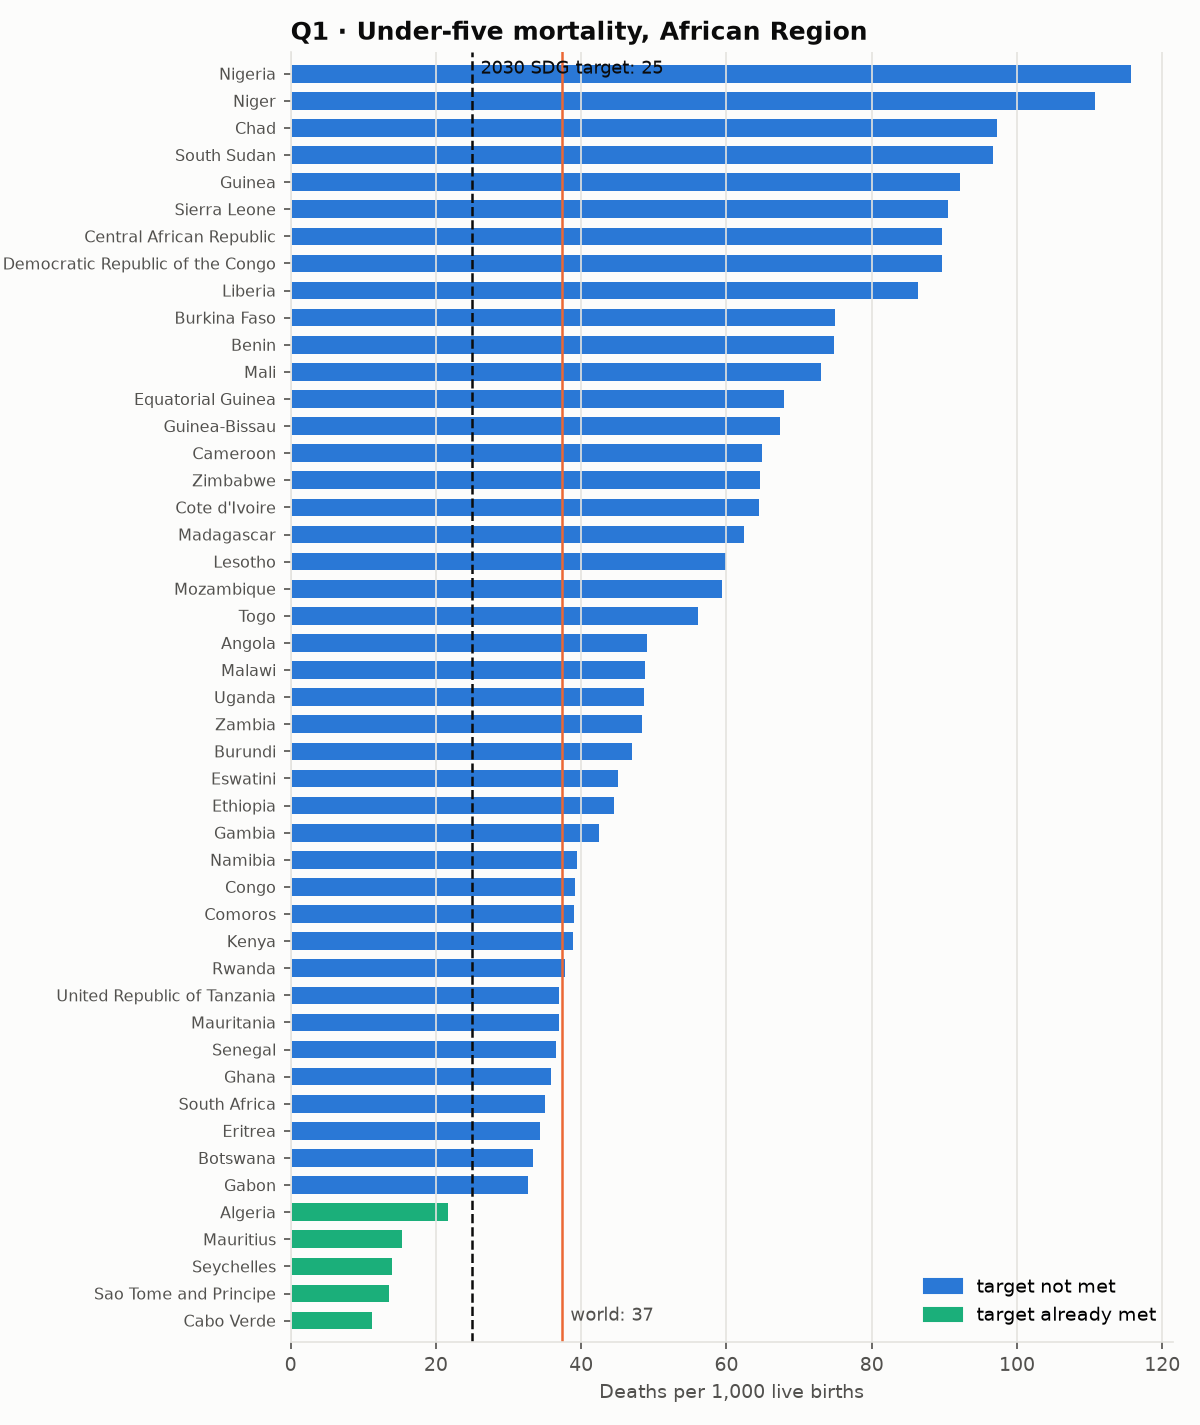
\includegraphics[width=0.78\linewidth]{q1_mortalite_moins_5_ans.png}
\caption{Under-five mortality by African Region country (2024)}
\end{figure}

\begin{figure}[H]
\centering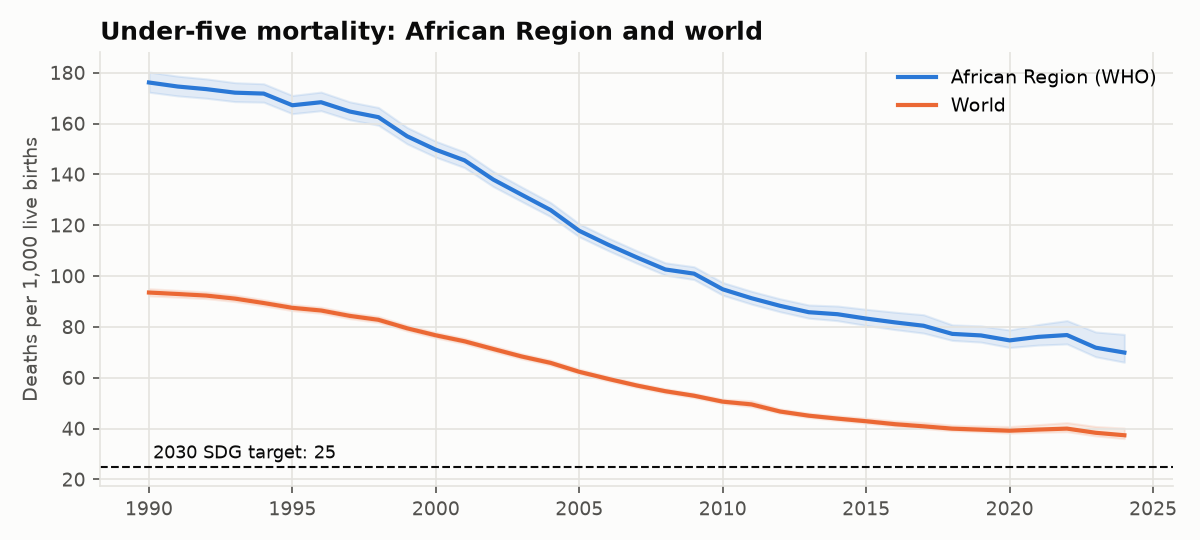
\includegraphics[width=0.92\linewidth]{q1_tendance_region_monde.png}
\caption{Trend since 1990, with uncertainty intervals}
\end{figure}

Under-five mortality in the region has fallen 2.5-fold since 1990, from 176 to 70 per 1,000. It remains nearly twice the global average.
The regional value (70) is well above the country median (48.7): the most populous countries, such as Nigeria (116), weigh heavily in the
regional total.

\subsection{Q2 · Which countries will meet the targets by 2030?}
Method: the \textbf{annual rate of reduction} (ARR) used by the UN Inter-agency Group for Child Mortality Estimation:
$\text{ARR} = \ln(v_{2015} / v_{t}) / (t - 2015)$, then a 2030 projection assuming that pace continues.

\begin{figure}[H]
\centering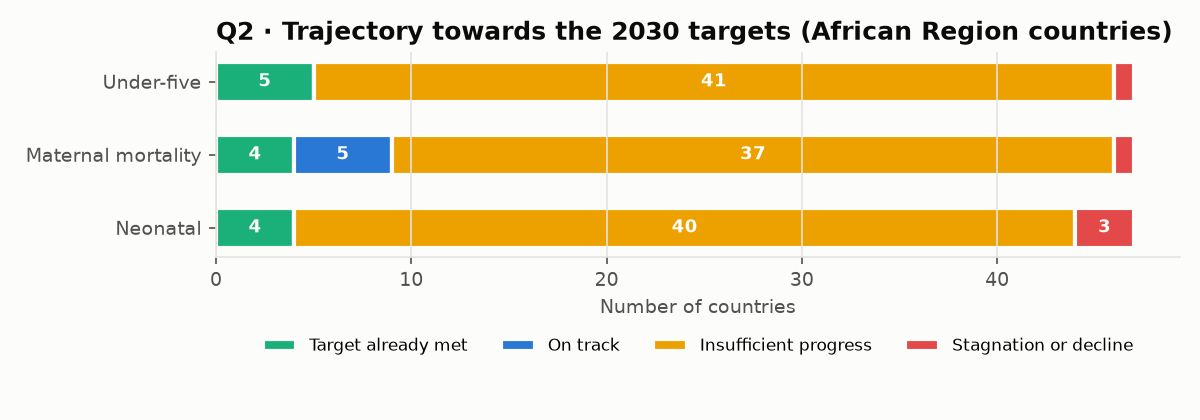
\includegraphics[width=0.92\linewidth]{q2_trajectoires_2030.png}
\caption{African Region countries by trajectory status}
\end{figure}

\begin{itemize}[leftmargin=1.2em]
  \item \textbf{Under-five mortality:} no off-target country is on track. The median country reduces mortality by \textbf{3.0\% a year}
        whereas \textbf{12.4\%} would be needed. Zimbabwe is going backwards (59.2 → 64.7 per 1,000 since 2015).
  \item \textbf{Maternal mortality:} the only target with countries on track: Eswatini, Mozambique, Namibia, Sao Tome and Principe and Zambia,
        with reductions of 7 to 11\% a year. Botswana is going backwards.
  \item \textbf{Neonatal mortality:} the slowest (1.7\% a year). It is stagnating or rising in Nigeria, South Africa and Zimbabwe.
\end{itemize}

\subsection{Q3 · How large is the gap between the poorest and richest households?}
\begin{figure}[H]
\centering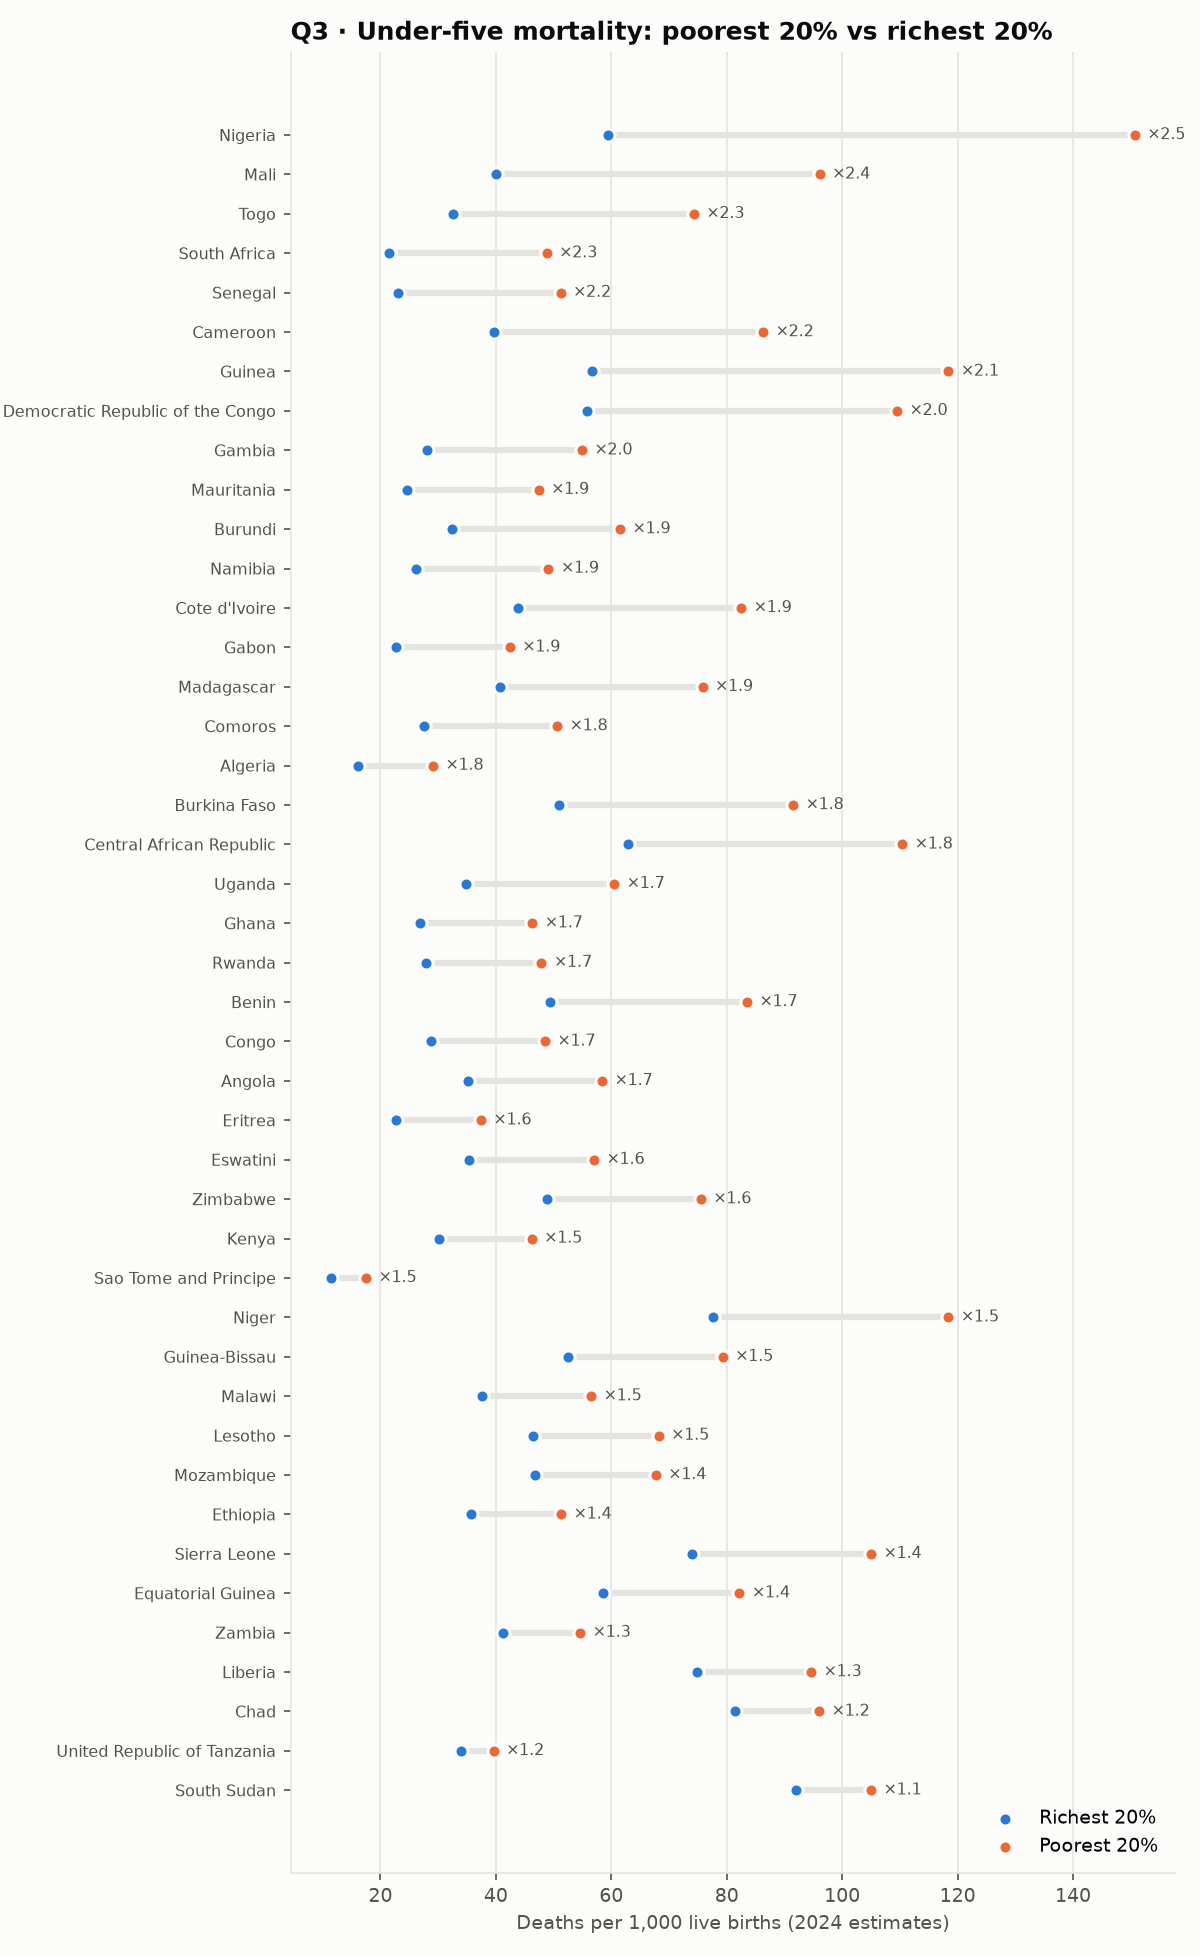
\includegraphics[width=0.74\linewidth]{q3_inegalites_richesse.png}
\caption{Under-five mortality: poorest 20\% vs richest 20\% (2024)}
\end{figure}

\begin{table}[H]
\centering\small
\begin{tabularx}{\linewidth}{@{}l r r r r@{}}
\toprule
\textbf{Year} & \textbf{Poorest 20\%} & \textbf{Richest 20\%} & \textbf{Absolute gap} & \textbf{Ratio} \\
\midrule
1990 & 186.6 & 118.8 & 63.3 & 1.56 \\
2000 & 159.7 & 94.2 & 50.5 & 1.49 \\
2015 & 74.4 & 46.3 & 28.2 & 1.67 \\
2024 & 61.5 & 37.6 & 23.2 & 1.71 \\
\bottomrule
\end{tabularx}
\caption{Medians across 43 African Region countries (deaths per 1,000 live births)}
\end{table}

A child born into the poorest 20\% of households is \textbf{1.7 times more likely} to die before age 5, and up to 2.5 times in Nigeria and
2.4 times in Mali. \textbf{The absolute gap has narrowed} from 63 to 23 per 1,000, but \textbf{the relative gap has widened since 2000}:
better-off households are improving proportionally faster.

\subsection{Q4 · Are inputs associated with outcomes?}
\begin{figure}[H]
\centering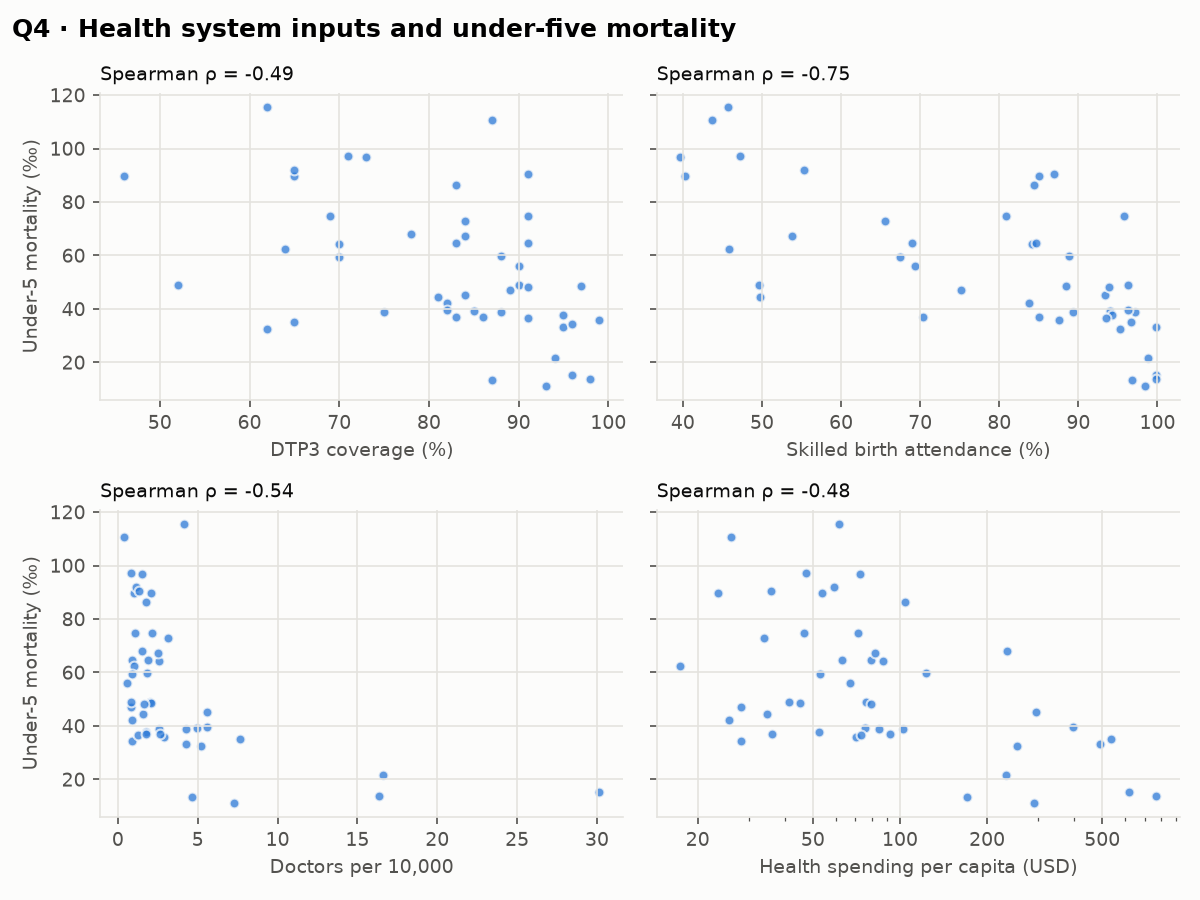
\includegraphics[width=0.86\linewidth]{q4_moyens_resultats.png}
\caption{Input indicators and under-five mortality (one dot = one country)}
\end{figure}

All inputs are associated with lower mortality, but with very different strength: \textbf{skilled birth attendance} ($\rho = -0.75$, 45 countries),
doctors ($-0.54$), DTP3 immunisation ($-0.49$), health spending ($-0.48$). These are \textbf{correlations}, not proof of causation: these inputs
also reflect countries' overall level of development.

\subsection{Recommendations to the board}
\begin{keybox}[For Initiative Baobab Santé]
\begin{enumerate}[leftmargin=1.4em]
  \item \textbf{Prioritise neonatal mortality:} it is the slowest-moving target (1.7\% a year). Deaths in the first month account for nearly
        half of under-five mortality (medians: 23.0 out of 48.7 per 1,000).
  \item \textbf{Explicitly target poor households:} the relative gap is widening. An untargeted programme benefits better-off households first.
  \item \textbf{Invest in skilled birth attendance:} it is the lever most strongly associated with low mortality in the region.
  \item \textbf{Study the countries on track} for maternal mortality (Mozambique, Zambia, Eswatini…) to draw lessons.
  \item \textbf{Re-run the pipeline after every WHO release:} revisions are now applied and tracked automatically.
\end{enumerate}
\end{keybox}

% =============================================================================
\section{Limitations and technical debt}\label{sec:limits}

\begin{tabularx}{\linewidth}{@{}L{5.4cm} Y@{}}
\toprule
\textbf{Limitation} & \textbf{Consequence} \\
\midrule
WHO data are modelled estimates & Uncertainty intervals are stored but not yet shown for each country \\
Linear pace projection (ARR) & Assumes the 2015–2024 pace continues until 2030 \\
Correlations (Q4) & They prove no causation \\
Country names in English & The WHO API does not publish French labels \\
\midrule
\multicolumn{2}{@{}l}{\textbf{Technical debt accepted at level 1}} \\
\midrule
Only the latest value is kept & Full revision history comes in project 2 \\
WHO deletions not handled & An observation withdrawn by WHO would remain in the database \\
No scheduling & Manual runs (orchestration in project 3) \\
No continuous integration & Tests are run by hand (CI/CD in project 3) \\
\bottomrule
\end{tabularx}

% =============================================================================
\section{Lessons learned}
\begin{itemize}[leftmargin=1.2em]
  \item \textbf{Grain first:} 8 ``identical'' values hid a dimension. Understanding the grain before modelling avoids the client's mistake.
  \item \textbf{Quality checks must be calibrated:} 25 ``outliers'' were real historical disasters.
  \item \textbf{Measure, don't guess:} 130\,s were lost in DNS resolution, not in the code.
  \item \textbf{Tests find real bugs:} the \texttt{None} / \texttt{NaN} trap would have emptied the database in production.
  \item \textbf{Check your own assumptions:} wealth data did not come from one-off surveys, and verifying it opened the question of how
        inequality has evolved.
\end{itemize}

% =============================================================================
\section{Roadmap}
\begin{tabularx}{\linewidth}{@{}L{4.6cm} Y@{}}
\toprule
\textbf{Improvement} & \textbf{Benefit} \\
\midrule
Revision history & History table (\emph{slowly changing dimension} type 2), planned for project 2 \\
Incremental loading & Download only updated indicators (WHO \texttt{Date} field) \\
Orchestration and CI/CD & Scheduled runs after each release, automatic tests on every change (project 3) \\
Dashboard & Interactive visualisation for the client's team, connected directly to PostgreSQL \\
\bottomrule
\end{tabularx}

% =============================================================================
\appendix
\section{SQL queries delivered}
\begin{tabularx}{\linewidth}{@{}L{5.2cm} Y@{}}
\toprule
\texttt{00\_schema.sql}, \texttt{01\_views.sql} & Schema (idempotent) and analysis views \\
\texttt{q0\_couverture\_donnees.sql} & Data coverage in the region \\
\texttt{q1\_cibles\_2030.sql} & Status against the targets \\
\texttt{q2\_rythme\_2030.sql}, \texttt{q2b\_…} & Trajectory by country and summary (ARR method) \\
\texttt{q3\_inegalites\_richesse.sql}, \texttt{q3b\_…} & Poor/rich gap, and its evolution since 1990 \\
\texttt{q4\_moyens\_resultats.sql} & Correlations between inputs and mortality \\
\texttt{controle\_recette.sql} & Acceptance checks (C2, C3, C4) \\
\bottomrule
\end{tabularx}

\section{Architecture decision records (ADR)}
\begin{tabularx}{\linewidth}{@{}l Y@{}}
\toprule
ADR 001 & Containerised PostgreSQL with Docker Compose, secrets in \texttt{.env} \\
ADR 002 & Staging and upsert loading, complete \texttt{NULLS NOT DISTINCT} business key \\
ADR 003 & Quality checks, quarantine and threshold calibration \\
\bottomrule
\end{tabularx}

\section{Glossary}
\begin{tabularx}{\linewidth}{@{}>{\bfseries}L{3.6cm} Y@{}}
SDG 3 & UN Sustainable Development Goal 3: ``Good health and well-being'' \\
Grain & What one row of a table represents \\
Staging & Transit area where a batch is loaded before being merged into the reference tables \\
Upsert & Insert if the row is new, update it if it exists \\
Quarantine & Table holding rows rejected by the checks, with their reason \\
ARR & Annual Rate of Reduction of an indicator \\
Wealth quintile & One fifth of the population ranked by household wealth (Q1: poorest 20\%) \\
Container & Isolated, reproducible environment running software, here PostgreSQL \\
\end{tabularx}

\end{document}
